\documentclass{paper}
%\usepackage{nomencl}
\usepackage{nomencl}
\usepackage{amsmath}
\usepackage{graphicx}
\usepackage{subfigure}
\usepackage{parskip}
%\usepackage{minted}
\usepackage[toc,page]{appendix}
\usepackage{csquotes}
\usepackage{framed}
\usepackage{amsthm}

\theoremstyle{theorem}
\newtheorem{theorem}{Theorem}[section]
 
\theoremstyle{definition}
\newtheorem{definition}{Definition}[section]

\theoremstyle{remark}
\newtheorem{remark}{Remark}[section]
%\usepackage{biblatex}
%\makenomenclature
\title{Introduction}
\author{A. Giavaras}
\date{}

\begin{document}
\maketitle
\tableofcontents

\clearpage
\section{Introduction to Self-driving Cars}
\label{introduction_self_driving_cars}
Self-driving cars promise to change everything related to automotive; road safety, mobility for everyone,  while dramatically reducing the costs of driving. 


In this series of notes, we'll introduce you to the self-driving car software and hardware architectures as well as the technologies involved in order to make
the autonomous driving concept a reality. The notes have been divided into the follwing broad sections:

\begin{enumerate}
\item Introduction to autonomous cars
\item State estimation, sensing, and localization for autonomous vehicles
\item visual perception, 
\item motion planning. 
\end{enumerate}

Concretely, after going over the material provided, you should be able to

\begin{enumerate}
\item design a basic hardware system for a self-driving car, 
\item identify the main components of the autonomous driving software stack, 
\item create a safety assessment strategy for self-driving car program. 
\end{enumerate}

You'll then learn to develop the complete model of a vehicles motion, define a PI controller for longitudinal control, define a path following controller for lateral vehicle control, and test out your control designs in a simulator. 

The second broad section is that of state estimation, sensing, and localization for autonomous vehicles. By the end of this section, you'll understand the key methods for perimeter and state estimation, develop and use models for typical vehicle localization sensors, apply extended and uncentered Kalman filters to a vehicle state estimation problem, and register point clouds created from LIDAR scans to a 3D map of a static environment. In the third section, we'll discuss about visual perception for self-driving cars. After completing the relevant material, you'll be able to project 3D points onto the camera image plane, calibrate the pinhole camera model, apply feature detection description and matching algorithms for localization and mapping, develop and train neural networks for both object detection and semantic segmentation. You'll apply these methods to vehicle tracking and drivable surface estimation. The fourth and final section deals with motion planning. There,  we'll teach you about motion planning for self-driving cars. By the end of this section, you'll be able to devise a trajectory roll out motion planning method, calculate the time to collision with static and constant velocity objects, plan routes over complex road networks, define high-level vehicle behaviors and transitions for vehicles navigating through intersections around parked cars and merging, and develop kinematically feasible paths through an environment with static obstacles, compute velocity profiles that satisfies speed, curvature and moving object motion planning constraints, plan behaviors and execute maneuvers to navigate safely through the world, and gain valuable experience in debugging and testing self-driving algorithms in the Carla simulator. 


So, by studing the material provided, you will have a detailed understanding of the architecture and components of the autonomous driving software stack and you will program your own self-driving car. 
Arguably, comprehension of the material has quite a number of prerequisites. In particular,

\begin{itemize}
\item you should be proficient in linear algebra and be familiar with matrices, vectors, matrix multiplication, rank, eigenvalues in vectors and inverses. This background will help you with control, state estimation, perception, and planning algorithms throughout the courses.
\item  You should also be comfortable with statistics. In particular, working with Gaussian probability distributions. This knowledge will be important for state estimation, and for perception when we're estimating vehicle speed and heading from GPS and inertial measurements for example. 
\item You should also be comfortable with basic calculus and physics, such as forces, moments, inertia, and Newton's laws.  
\end{itemize}

If you don't have these necessary pre-requisites, there are excellent robotics, AI, deep learning, and other courses that you can take on Coursera to prepare you for this specialization. Autonomous driving is a constantly evolving and changing field. So, keeping up not only with self-driving knowledge but also robotics, AI, and deep learning will help you keep your technical skills sharp. 
There's a long way to go, and we need pioneers to help us get there. So, are you ready for the ride?


\subsection{Basic Terms}

In this section you will learn about the main components needed to create a self-driving car and the technical requirements that drive their design. 
However, before we begin, it's important that you understand autonomous vehicle requirements or how we define self-driving for a car. 
Thus let's  first begin with a high level survey of the terms and concepts that we'll explore more deeply throughout these notes. So in this section one, we will introduce  
the taxonomy for self-driving cars or a system of classification that we use to define driving automation. Next, we'll describe the perception needs for the driving task or those items that we need to be able to identify properly. Finally, we will tackle the question of how to make driving decisions and discuss a few approaches for making choices about how a vehicle moves through the environment. 
The goal of this first module is to remind you just how many assessments and decisions the driving task truly requires. Hopefully this will help you appreciate just how much complexity we as humans can manage effectively when it comes to staying safe on the road. 

Let's get started with some technical terms and definitions.  The first term on our list is the {\textbf{driving task}}. Broadly speaking, the driving task is made up of three sub-tasks. 

\begin{enumerate}
\item Perception, or perceiving the environment that we're driving in. This includes tracking a car's motion in identifying the various elements in the world around us, like the road surface, road signs, vehicles, pedestrians and so on. We also need to track all moving objects and predict their future motions. So we can drive safely and accurately. 
\item The second sub-task is motion planning. This allows us to reach our destination successfully. For example, you may want to drive from your home to your office. So you'll need to consider which roads you should take, when you should change lanes or cross an intersection and how to execute a swerve maneuver around a pothole along the way. 
\item The third is vehicle control. We need to take the appropriate steering, break and acceleration decisions to control the vehicle's position and velocity on the road. 
\end{enumerate}

These three sub-tasks form the main driving task and need to be performed constantly while driving a vehicle. The next concept I'll introduce, is called the {\textbf {Operational Design Domain or ODD}} for short. The ODD constitutes the operating conditions under which a given system is designed to function. It includes environmental, time of day, roadway and other characteristics under which the car will perform reliably. Clearly defining the operating conditions for which a self-driving car is designed, is crucial to ensuring the safety of the system. So the ODD needs to be planned out carefully in advance. 

\subsection{Taxonomy of Driving}
\label{driving_taxonomy}

Now that we know some of the basic terms, let's get to the big question. How do we classify the level of automation in a driving system? 
Here are some things to consider. First how much driver attention is needed? For example, can you watch a movie while driving to work? Or do you need to keep your attention on the steering wheel at all times? Driver attention is one of the crucial questions to consider when defining the level of autonomy. Second, how much driver action is actually needed? For example do you need to steer? Does the car take care of the speed or do you control that as well? Do you need to change lanes or can the car stay in the current lane without any intervention? What exactly do we need to expect when we say that the car can automatically drive? Although we defined the driving task broadly previously, we will need to discuss this in more depth. 

All of these questions lead us to the autonomous driving taxonomy. The standards are continuously evolving but for the purposes of our classification, we will use the decomposition suggested by the Society of Automotive Engineers in 2014, see \cite{SAE2014, SAE2016}. Let's now discuss a way to describe the driving task in increasing levels of automation. 

First, we have lateral control which refers to the task of steering and navigating laterally on the road. Turning left, right, going straight or tracking a curve and so on. Next we have longitudinal control. This is the task where we control the position or velocity of the car along the roadway, through actions like breaking or acceleration, see figure \ref{lateral_longitu_control}. 


\begin{figure}[!htb]
\begin{center}
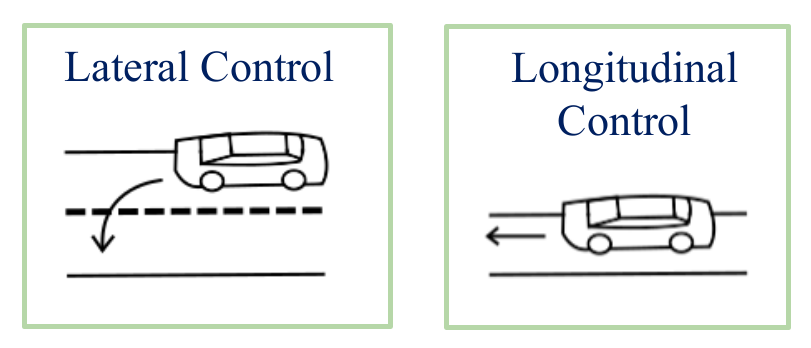
\includegraphics[scale=0.280]{img/intro_self_driving/lateral_longitu_control.jpeg}
\end{center}
\caption{Schematics of lateral and longitudinal motion.}
\label{lateral_longitu_control}
\end{figure}


Then we have {\textbf{Object and Event Detection and Response or OEDR}} for short. 
OEDR is essentially the ability to detect objects and events that immediately affect the driving task and to react to them appropriately. 
OEDR really encompasses a large portion of autonomous driving. 
It is used in conjunction with the specific Operational Design Domain to categorize current self-driving systems. 
Next we have planning. Planning is another important aspect of driving. As immediate response is already part of OEDR, planning is primarily concerned with the long and 
short term plans needed to travel to a destination or execute maneuvers such as lean changes and intersection crossings. 
Finally, there are some miscellaneous tasks that people do while driving as well. 
These include actions like signaling with indicators, hand-waving, interacting with other drivers and so on. 
Now we have a clear description of what tasks we expect a self-driving car to perform. Let's now discuss the questions that can lead us to the taxonomy for classifying the 
level of automation in a self-driving car. 

First, can this system handle steering tasks or lateral control? Second, can it perform acceleration, braking and velocity manipulation tasks or longitudinal control? 
Third, can the system perform object and event detection and response and to what degree? Crucially, can the system handle emergency situations by itself or does it always 
need a driver to be attentive during emergencies? Finally, can the system perform in all scenarios and all conditions? Or does it have a limited ODD or set of operating conditions that 
it can handle safely? 

Based on these questions let's walk through the commonly-used levels of automation defined by the SAE Standard J3 016 \cite{SAE2016}. 
Let's start with full human perception, planning and control and call this level 0. In this level, there is no driving automation whatsoever and everything is done by the driver. 
If an autonomous system assist the driver by performing either lateral or longitudinal control tasks, we are in level one autonomy. Adaptive cruise control is a good example of level one. 
In adaptive cruise control or ACC, the system can control the speed of the car. 
But it needs the driver to perform steering. Hence, it can perform longitudinal control but needs the human to perform lateral control. 
Similarly, lane keeping assist systems are also Level one. 
In lane keeping assistance, the system can help you stay within your lane and warn you when you are drifting towards the boundaries. 
Nowadays, systems rely on visual detection of lane boundaries coupled with lane centering lateral control. Let's move on to the next level, the level of partial automation. 
In level two the system performs both the control tasks, lateral and longitudinal in specific driving scenarios. Some simple examples of level two features are GM Super Cruise and Nissan's Pro Pilot Assist. These can control both your lateral and longitudinal motion but the driver monitoring of the system is always required. 
Nowadays, many automotive manufacturers offer level two automation products including Mercedes, Audi, Tesla and Hyundai. Next up is level three. In level three or the level of conditional automation, 
the system can perform Object and Event Detection in Response to a certain degree in addition to the control tasks. 
However, in the case of failure the control must be taken up by the driver. 
The key difference between level two and three, is that the driver does not need to pay attention in certain specific situations, as the vehicle can alert the driver in time to intervene. 
This is a controversial level of automation as it is not always possible for an autonomy system to know when it is experiencing a failure. 
An example of level three systems, would be the Audi A Luxury Sedan, which was an automated driving system that can navigate unmonitored in slow traffic. 
In the next level, we arrive at highly automated vehicles, where the system is capable of reaching a minimum risk condition, in case the driver doesn't intervene in time for an emergency. 
Level four systems can handle emergencies on their own but may still ask drivers to take over to avoid pulling over to the side of the road unnecessarily. 
With this amount of automation, the passengers can check their phone or watch a movie knowing that the system is able to handle emergencies and is capable of keeping the passengers safe. 
However, level four still permits self-driving systems with a limited ODD. As of fall 2018, only Waymo has deployed vehicles for public transport with this level of autonomy. The Waymo fleet can handle the driving task in a defined geographic area with a nominal set of operating conditions, without the need for a human driver. 
Finally, in level five the system is fully autonomous and its ODD is unlimited. 
Meaning that it can operate under any condition necessary. 

Level five is the point where our society undergoes transformational change. With driverless taxis shuttling people in packages wherever we need them. 
We don't have any examples for level five yet. 


\begin{framed}
\theoremstyle{remark}
\begin{remark}{\textbf{Taxonomy of Driving}}

The aforementioned levels of autonomy are actually a coarse measure of automation. 
In fact, it is possible for two car models to claim level four autonomy but have very different capabilities in ODDs. 
Furthermore, albeit a given vehicle may be equipped with a driving automation system that is capable of delivering multiple driving automation 
features that perform at different levels, the level of driving automation exhibited in any given instance is determined by the feature(s) that are engaged.
\end{remark}
\end{framed}


\begin{figure}[!htb]
\begin{center}
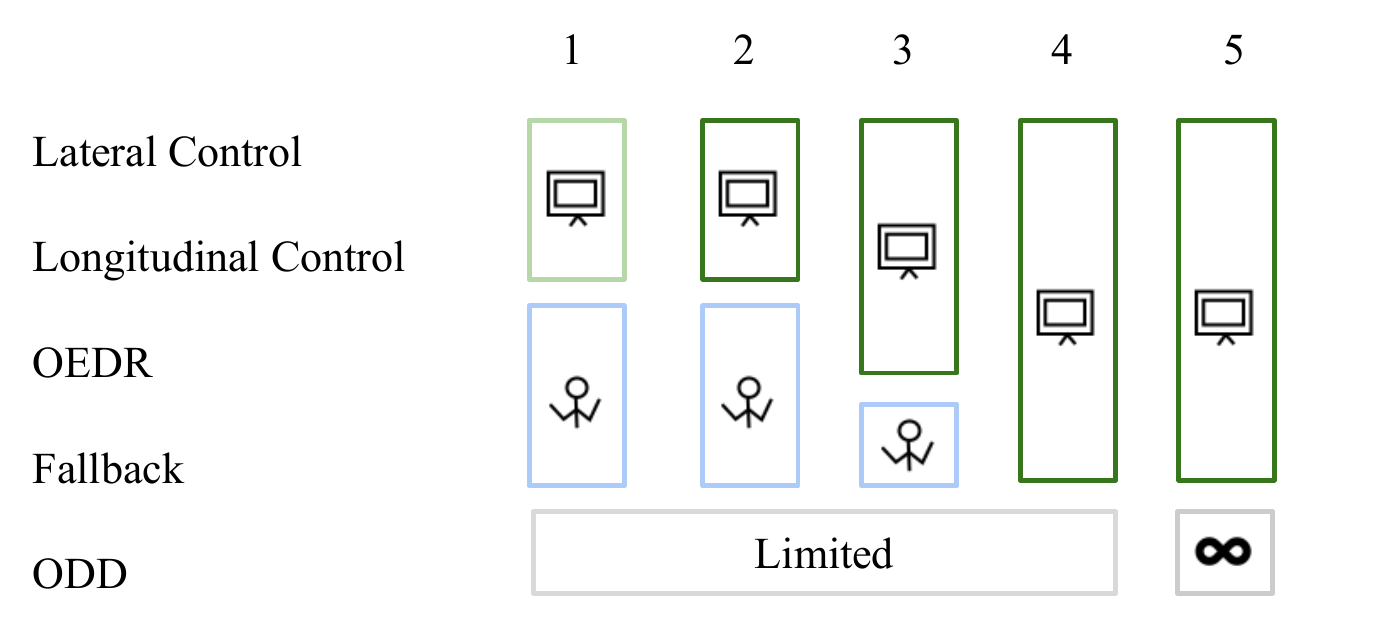
\includegraphics[scale=0.280]{img/intro_self_driving/levels_of_automation.jpeg}
\end{center}
\caption{Levels of automation.}
\label{levels_of_automation}
\end{figure}

\begin{framed}
\theoremstyle{remark}
\begin{remark}{\textbf{Primary actors in driving}}

There are three primary actors in driving: 

\begin{enumerate}
\item The (human) user
\item The driving automation system
\item Other vehicle systems and components.
\end{enumerate}
\end{remark}
\end{framed}


\subsection{Questions}
\label{introduction_self_driving_cars_questions}

\begin{enumerate}

\item Which of the following are components of longitudinal control? (Select all that apply)
\begin{enumerate}
\item Braking
\item Steering
\item Accelerating
\item Planning
\end{enumerate}

\item Which of the following is not an example of OEDR?

\begin{enumerate}
\item Stopping at red light
\item Finding a route from your location to a goal location
\item Slowing down when seeing a construction zone ahead
\item Pulling over upon hearing sirens.
\end{enumerate}

\item Which of the following tasks would you expect a Level 2 system to perform? (Select all that apply)

\begin{enumerate}
\item Maintain constant speed
\item Change lanes
\item Stay within a lane
\item Swerve and slow down to avoid a pedestrian
\end{enumerate}

\item What is the distinction between Level 3 autonomy and Level 4 autonomy? 


\begin{enumerate}
\item Level 3 systems only have lateral or longitudinal control. Level 4 systems have both.
\item Level 3 systems cannot drive on highways. Level 4 systems can.
\item Level 3 systems cannot perform OEDR. Level 4 systems can.
\item Level 3 systems require full user alertness. Level 4 systems do not.
\end{enumerate}

\item What distinguishes Level 5 Autonomy from Level 4?


\begin{enumerate}
\item Level 5 autonomy can operate on any weather condition. Level 4 cannot.
\item Level 5 autonomy has OEDR capability. Level 4 has not.
\item Level 4 has restricted operational design domain. Level 5 is unrestricted.
\item Level 5 autonomy can operate on any road surface and road type. Level 4 cannot.
\end{enumerate}

\end{enumerate}


\section{Perception}
\label{perception}
In the previous section, we learned how to classify automation according to its capabilities and operational design domain. 
In this section, we will start analyzing how a driving task is performed. Specifically, we will go over the many processes of perception. 
We will first define the perception task, listing out the requirements for perceptions such as what static and dynamic objects we need to identify, 
and what needs we have for tracking the ego vehicles motion through the environment. 
Finally, we will conclude with a discussion on some challenges to robust perception. So let's get started.


Very roughly speaking, any driving tasks can be broken down into two components, figure \ref{driving_task}. 

\begin{figure}[!htb]
\begin{center}
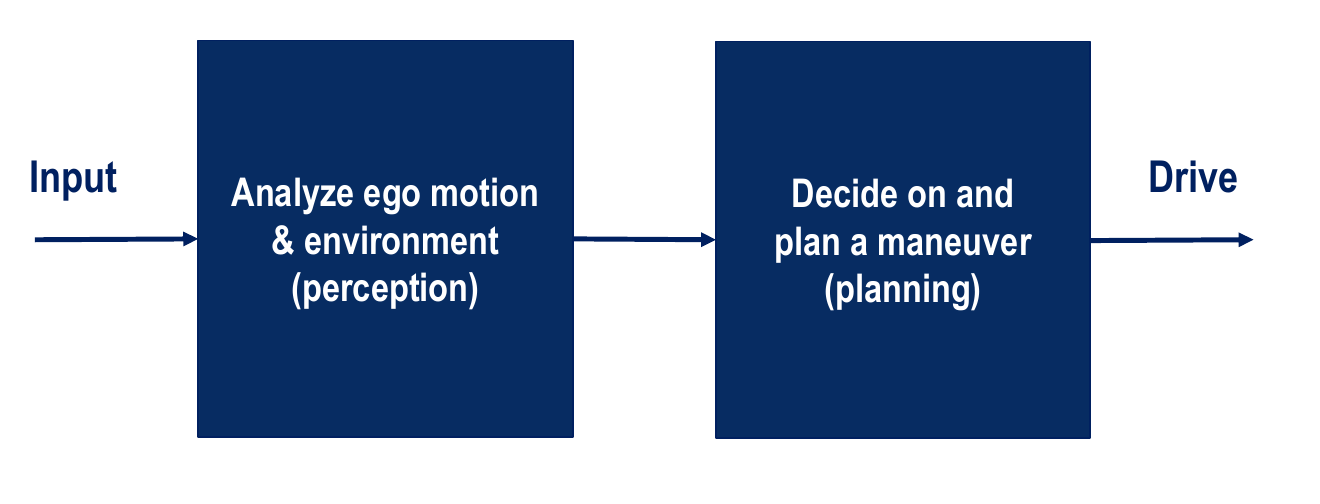
\includegraphics[scale=0.280]{img/intro_self_driving/driving_task.jpeg}
\end{center}
\caption{Schematics of the driving task as I/O process.}
\label{driving_task}
\end{figure}

First, we need to understand what's happening around us and where we are. So, we need to perceive our surroundings. 
Secondly, we need to make a driving decision. For example, should we accelerate or stop before a pedestrian about to enter the roadway? 
Recall from the previous section the concept of OEDR or object and event detection and response. 
Any driving task requires some kind of OEDR, that is, we need some way of identifying objects around us, recognizing events happening near us, and then responding to it. 
Recall that the classification of automated systems that we discussed had OEDR as one of the criteria. 
In other words, if we want to build a self-driving car, we need to be able to perform OEDR. Let's go further and analyze a crucial part of OEDR perception. 

\subsection{What is perception?}
So, what is perception? As we discussed, we want to be able to make sense of the environment around us and the way we're moving within it. 
In particular, for any agent or element on the road, we need to first identify what it is; a car, a cyclist, a bus, etc. 
On a second stage, we want to understand its motion; has it been moving in a certain way that can tell us what it will do next. 
As humans, we're really good at understanding patterns. 
However, it's still difficult for computer systems to be able to recognize these same patterns around us as quickly as we do. 
We can point to a car going straight and say, "Oh, it will be in this position in some amount of time in the future." 
This is what makes driving possible for us. So, this ability of predicting the trajectory of a moving object is really important to perception. 
If we can do this prediction correctly, we can make informed decisions. For example, if I know what the car in front of me is going to do next, 
then I can decide what to do next in such a way that both of our goals are met. 

Let's discuss the various elements we need to be able to identify for the perception task. 
First, we need to identify static elements. These are elements like roads and lane markings, things that segregate regions on the roads like zebra crossings, 
and important messages such as school up ahead. These are all on the road area, see figure \ref{static_objects}.

\begin{figure}[!htb]
\begin{center}
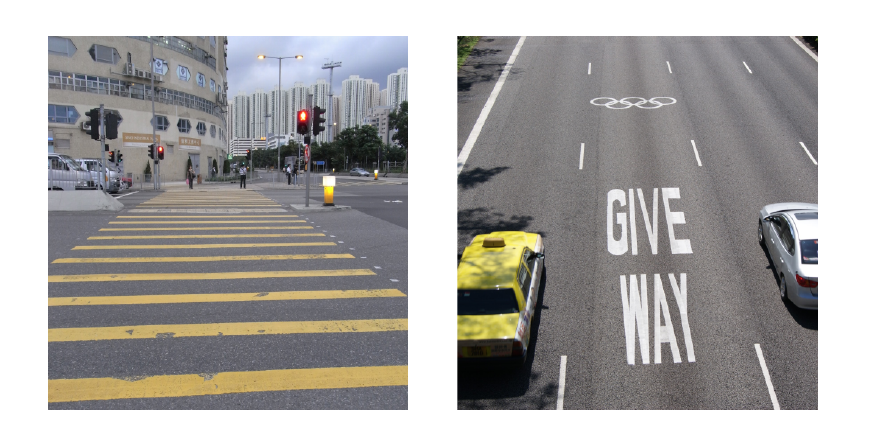
\includegraphics[scale=0.280]{img/intro_self_driving/static_objects.jpeg}
\end{center}
\caption{Lane markings and zebra crossings.}
\label{static_objects}
\end{figure}

Then there are off-road elements like curbs that define the boundaries within which we can drive. 

\begin{figure}[!htb]
\begin{center}
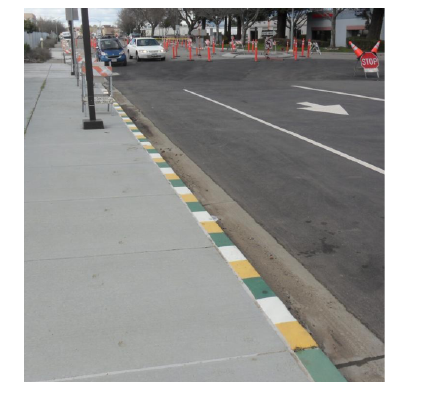
\includegraphics[scale=0.280]{img/intro_self_driving/static_objects_2.jpeg}
\end{center}
\caption{Off road signals.}
\label{static_objects_2}
\end{figure}

There are the on-road traffic signals that periodically change and signal whether you are allowed to move forward, or left, or right, or just stay stopped. 
Then there are all kinds of road signs like those telling you the speed limit, indicating direction, whether there is a hospital coming up, or a school coming up, and so on. 

\begin{figure}[!htb]
\begin{center}
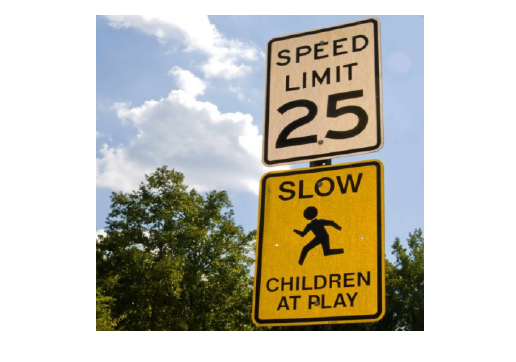
\includegraphics[scale=0.280]{img/intro_self_driving/road_signs.jpeg}
\end{center}
\caption{Road signs.}
\label{road_signs}
\end{figure}

Again, these are off-road elements. Finally, there are road obstructions. So, the orange cones that tell you construction is happening or that there is roadblock edge and so on, see figure \ref{construction_signs}. Also, these are on road elements. 


\begin{figure}[!htb]
\begin{center}
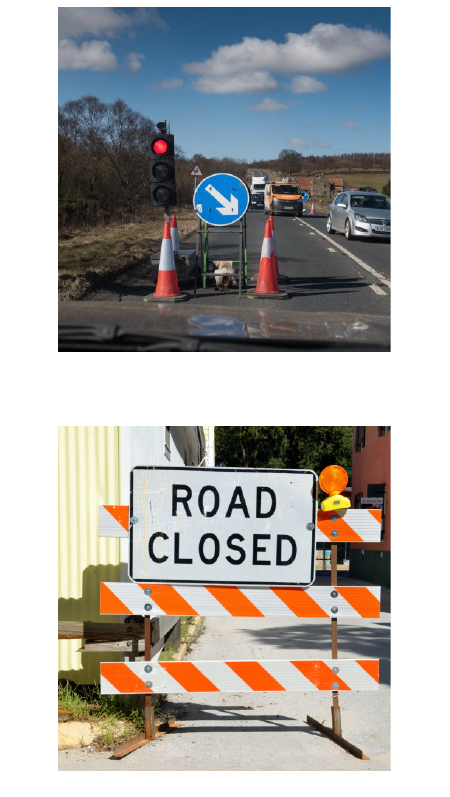
\includegraphics[scale=0.280]{img/intro_self_driving/construction_signs.jpeg}
\end{center}
\caption{Construction signs.}
\label{construction_signs}
\end{figure}

All the above can be classified as static elemens. Let's discuss the dynamic elements that we need to identify for perception. 
These are the elements whose motion we need to predict to make informed driving decisions. 
We need to identify other vehicles on the road, so four wheelers like trucks, buses, cars, and so on, and then we also need to identify and predict the motion of two wheelers, like motorcycles, bicycles, and so forth. These are all moving systems with more freedom than four wheelers, and so they are harder to predict. 
Finally, we should also be able to identify and predict the motion of pedestrians around us. 
How pedestrians behave is very different from vehicles as pedestrians are known to be much more erratic than vehicles in their motion because of the inherent freedom that humans have in the way they move. Another crucial goal for perception is ego localization. 
We need to be able to estimate where we are and how we are moving at any point in time. 
Knowing our position and how we are moving in the environment is crucial to making informed and safe driving decisions. 
The data used for ego motion estimation comes from GPS, IMU, and odometry sensors, and needs to be combined together to generate a coherent picture of our position. 
 

Now that we've discussed the main goals for perception, let's conclude this discussion by going over why perception is also a difficult problem. First, performing robust perception is a huge challenge. Detection and segmentation can be approached with modern machine learning methods, but there is much ongoing research to improve the reliability and performance to achieve human level capability. Access to large datasets is critical to this effort. 
With more training data, our segmentation and detection models perform better and more robustly, 
but collecting and labeling data for all possible vehicle types, weather conditions, and road surfaces is a very expensive and time-consuming process. 
Second, perception is not immune to censor uncertainty. There are many times that visibility can be challenging, or GPS measurements get corrupted, or LIDAR and Radar returns are noisy in terms of their position value. Every subsystem that relies on these sensors must take uncertain measurements into account. 
This is why it is absolutely crucial to design subsystems that can accommodate sensor uncertainty and corrupted measurements in every perception task. 
Then there are effects such as occlusion and reflection in camera or LIDAR data. 
These can confuse perception methods with ambiguous information that is challenging to resolve into accurate estimates of object locations. 
There are also effects such as drastic illumination changes and lens flare, or GPS outages and tunnels which makes some sensor data completely unusable or unavailable. 
Perception methods need multiple redundant sources of information to overcome sensor data loss. 
Finally, there's weather and precipitation that can adversely affect the quality of input data from sensors. 
So, it is crucial to have at least some sensors that are immune to different weather conditions, for example radar. 


\subsection{Questions}
\label{perception_questions}

\begin{enumerate}

\item Which of the following tasks are associated with perception? (Select all that apply) 
\begin{enumerate}
\item Estimating the motion of other vehicles
\item Identifying road signs
\item Responding to traffic light changes
\item Plannning routes on a map
\end{enumerate}

\item Which of the following can be on road objects? (Select all that apply) 

\begin{enumerate}
\item Potholes
\item Stop signs
\item Sidewalks
\item Vehicles
\end{enumerate}

\item Which of the following tasks pose challenges to perception? (Select all that apply) 

\begin{enumerate}
\item Having sensors work in adverse weather conditions
\item Having sensor occlusion and reflection
\item Handling sensor uncertainty
\item Detecting tracking and predicitng dynamic object motions
\end{enumerate}

\item Which of the following sensors are used for ego localization? (Select all that apply) 


\begin{enumerate}
\item Global Navigation Satellite System GNSS
\item Radar
\item Barometers
\item Inertial Measurement Unit (IMU)
\end{enumerate}

\item Which of the following objects would be relevant for perception in adaptive cruise control?


\begin{enumerate}
\item Road signs
\item Traffic lights
\item Other vehicles
\item Lane markings
\end{enumerate}

\end{enumerate}


\section{Driving Decisions}
\label{driving_decisions}
In this section, we will be discussing decision-making in a self-driving car system. 
In the previous section, we discussed the concept of perception which forms the first step in performing a driving task. 
The other steps in driving include decision-making and then, finally, executing the decisions. 
In this section, we will categorize planning informally on the basis of the window of time over which the decision has to be made and discuss some examples. 
Then we will go over a simple intersection scenario and try to list out some of the various decisions needed to complete the driving task successfully. 
We will then categorize planning formaly based on the type of logic we use to make the decisions. 
So, is our logic made up of well-defined rules that react only to currently available information about the driving environment? 
Or is it also dependent on trajectory predictions of other agents? Let's get started. 


Making driving decisions falls under the bigger umbrella of planning. When we make driving decisions, we usually have three kinds of decisions to make. 

\begin{itemize}
\item Long-term planning decisions. A question such as, how do I navigate from New York to Los Angeles or from my home to work? By answering this question, we have a mission plan, a high-level plan for the entire driving task. Mapping applications that you use today are able to give you these driving instructions: which roads to take, which lanes to be in, and so on. But driving needs much more than that. 
\item Short-term driving decision with questions like, is it safe to change lanes now? Or when should I execute a left turn at an intersection? 
\item immediate decisions or reactions. These decisions involve control and trajectory planning and answer questions like, how do I follow my lane on this curved road? 
What steering input should I apply? Should I accelerate or brake? If so, by how much.
\end{itemize} 


\subsection{Intersection Scenario}

Let's discuss a very simple example of a driving task and try to think about what kind of decisions are involved. Suppose you are approaching an intersection on your way home. 
The long-term planning stage requires you to turn left at this intersection. 
Now, let's look at the intermediate and short-term decisions that need to be made. 
First, let's assume that the intersection is controlled. 
That is, it has traffic lights. Since you are turning left, you have to identify if you need to make a lane change into a left turning lane. 
Then, as you're approaching this intersection, you choose to slow down, and to do so smoothly so that the passengers don't experience discomfort. 
Nobody likes a jerky driver after all. You then come to a stop just before the stop line, before a pedestrian crossing. 
These decisions on lane changes and stopping locations are all short-term planning decisions. 
However, we also need to think and respond to situations that arise along the way. 
We still need object and event detection and response. 
What if a vehicle pulls into the turn lane in front of you? You would want to stop earlier to make room for the other vehicle. 
What if the stop lines weren't marked? You would have to approximately judge where the implied stop line is and stop before the pedestrian crossing. 
What if there were other vehicles behind you or even stalled in the intersection? 
How does the decision to execute a left turn change based on the many possible scenarios that can rapidly arise in normal driving? 
All of these decisions fall into the immediate decision category and requires safe reactions from the planning system. 
The end result is an exploding list of possible decisions to evaluate on different timescales, even for a simple left turn scenario. 
This amounts to talking about different cases for the same intersection crossing or scenarios. 
In each scenario, we need a consistent set of choices to be evaluated in real time and updated as new information about the scene becomes available. 
Furthermore, because decisions to change lanes affect where to drive and which cars to regulate our position relative to, 
even a seemingly simple driving scenario requires three or four levels of decisions, and must then still be executed with careful vehicle control. 
This example is really only scratching the surface of the constant stream of decisions needed for motion planning. 
The bottom line is, driving is complicated. Let's go ahead and discuss a possible structure to represent these decisions in software. 


{\textbf{Reactive planning}}

One method to address the challenge of multilevel decision-making is reactive planning. 
In reactive planning, we define sets of rules that take into account the current state of the ego vehicle 
and other objects in the environment and produce immediate actions. 
So, these are rules that only consider the current state and not future predictions. 
Some examples of such rules would be, if there is a pedestrian on the road, stop. 
Or if the speed limit changes, adjust your speed to match it. 
In both of these rules, we just observe what is happening right now and make our decision based on immediately available information. 
But there are other kinds of planning as well. 

{\textbf{Predictive planning}}

In predictive planning, we make predictions on how other agents in the environment, like vehicles and pedestrians, will move over time. 
We use this current state and prediction information to define all of our decisions. 
Some examples of rules in predictive planning would be, that car has stopped for the last 10 seconds. 
It's probably going to stay stopped for the next few seconds. 
So, perhaps there is a way that I can move past it safely. 
Or a pedestrian is jaywalking. 
They will enter our lane by the time I get close to them. Let me slow down and give them a chance to cross the road ahead of me. 
As you can see, this is a more natural way to think, and relates closely to how humans operate vehicles. 
We predict where other objects on the road will be in the future before we make our decisions. 
This type of planning, however, relies on accurate predictions of the actions of the other 
actors in the environment, which adds a significant layer of complexity to the perception tasks. 
Nonetheless, predictive planning is the predominant method for self-driving cars, as it greatly expands the scenarios a vehicle can handle safely. 


Let's summarize this section. We discussed the planning problem and the different types of planning based on the window of time over which we have to act. 
These types are long-term, short-term, and immediate planning. 
Then we discussed a simple intersection scenario, where we had to make a left turn. 
We concluded that driving is a really hard problem since we have so many variables and possibilities that result. 
Then we discussed two different planning approaches: reactive planning and predictive planning. 
This is just the tip of the iceberg. There's clearly so much more we need to think about before making a decision during the driving task. 
 
Let's quickly recap what we learned this week. In this module, we explored the basic autonomous driving terminology that's useful for later weeks of the specialization. We then discussed the levels of automation, and came up with a taxonomy to characterize self-driving capabilities. Then we define the driving task and the major components of driving: perception, planning, and execution. We then listed the elements and agents in the environment we need to identify and track for perception. We also discussed why perception is so hard. Then we discussed planning with its different horizons, and looked at some decision-making approaches. In the next module, we will define the main components of self-driving cars, including both the hardware and software elements that make up a complete system. See you then.


\section{Review Questions}
\label{review_questions_chapter_1}



\begin{enumerate}

\item You’re at home and need to drive to work. During the trip, you will be performing OEDR tasks. Of the tasks below, which of the following is not an example of OEDR? 
\begin{enumerate}
\item Stopping at a red light
\item Slowing down when seeing a construction zone ahead
\item Maintaining a distance to a vehicle ahead
\item Pulling over upon hearing sirens
\end{enumerate}

\item Which of the following tasks are associated with perception? 

\begin{enumerate}
\item Identifying road signs
\item Respond to traffic lights
\item Planning routs on a map
\item Estimating the motion of other vehicles
\end{enumerate}

\item Before leaving, you decide to check the weather. The forecast states that over the next few days there will be both sun and rain along with some fog. Assuming your vehicle exhibits Level 5 autonomy, which of the following weather conditions can your vehicle operate

\begin{enumerate}
\item Clear and sunny
\item Windy heavy rainfall
\item Heavy fog
\item Light rainfall
\item all of the above
\end{enumerate}

\item You enter your autonomous vehicle and it drives your usual route to work. While the vehicle is driving, you decide to take a nap. For which levels of autonomy is this safe? (Select all that apply) 


\begin{enumerate}
\item 1
\item 2
\item 3
\item 4
\item 5
\end{enumerate}

\item You’re approaching an all ways stop sign and you want to make a right turn. Your vehicle is denoted in orange. There are 2 pedestrians currently crossing and another vehicle (denoted in green) approaching the stop sign from the left

\begin{figure}[!htb]
\begin{center}
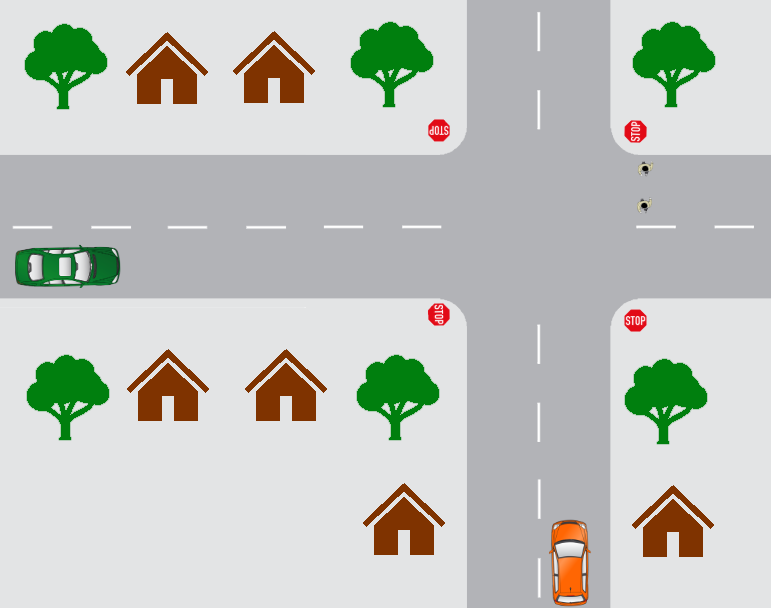
\includegraphics[scale=0.280]{img/intro_self_driving/summary_question_scenario_2.png}
\end{center}
\caption{Road signs.}
\label{summary_question_scenario_2}
\end{figure}

This task involves multiple considerations, which of them are predictive planning? Select all that apply

\begin{enumerate}
\item At a stop sign, stop and look both ways before proceeding
\item Gradually decelerate while reaching the stop sign
\item The green car arrives at the stop sign after you and plans to travel straight through the intersection. 
You choose to move first
\item Wait for the pedestrians to finish crossing before turning
\end{enumerate}


\item Here are some rules for driving at a stop sign. 


\begin{itemize}
\item For non all-way stop signs, stop at a point where you can see oncoming traffic without blocking the intersection
\item If there are pedestrians crossing, stop until they have crossed
\item If you reach a stop sign before another vehicle, you should move first if safe
\end{itemize}

Which of the following is an appropriate priority ranking?

\end{enumerate}


\section{Output Feedback}
\label{output_feedback}

Chapter \ref{state_feedback} introduced the concept of reachability. It was shown that it is possible to find 
a state feedback law that gives the desired closed loop eigenvalues provided that the system
is reachable.  Furthermore, we saw how to design controllers using
the system state, $x(t)$, as feedback to out controller. 

However, desigining state feedback controllers preassumes that all the states are measured. For many situations, it
is highly unrealistic to assume that all the states are measured. 

In this section we proceed somehow in a similar vein we can use the output $y(t)$ to modify the dynamics of the system through the use of observers. Furthermore, we will introduce the concept of observability
and show that if a system is observable, it is possible to recover the state
from measurements of the inputs and outputs to the system. We then show how to
design a controller with feedback from the observer state. 




\section{Observability}
\label{observability}

For many situations, it is highly unrealistic to assume that all the states are measured. In this section we
investigate how the state can be estimated by using a mathematical model and a
few measurements. It will be shown that computation of the states can be carried
out by a dynamical system called an \textbf{observer}, see also figure \ref{observer_block_diagram}.


\begin{framed}
\theoremstyle{definition}
\begin{definition}{\textbf{Observability}}
A linear system is \textbf{observable}  if for any $T>0$ it is possible to determine the state of the system $x(T)$ through measurements of $y(t)$ and $u(t)$ on the interval $[0,T]$  $x(T) = x_f$.
\end{definition}
\end{framed}


\begin{framed}
\theoremstyle{remark}
\begin{remark}{\textbf{Nonlinear Systems}}

The definition above holds for nonlinear systems as well, and the results discussed here have extensions to the nonlinear case.
\end{remark}
\end{framed}


Consider again the system

\begin{equation}
\frac{dx}{dt} = Ax + Bu ~~ y = Cx + Du
\end{equation}


where $x\in R^n$ is the state, $u\in R^{p}$ is the input and $y\in R^q$ the measured output.

We wish to estimate the state of the system from its inputs and outputs, as illustrated
in Figure \ref{observer_block_diagram}. In some situations we will assume that there is only one measured
signal, i.e., that the signal $y$ is a scalar and that $C$ is a (row) vector. This signal may
be corrupted by noise $n$, although we shall start by considering the noise-free case.
We write $\hat{x}$ for the state estimate given by the observer.

\begin{figure}[!htb]
\begin{center}
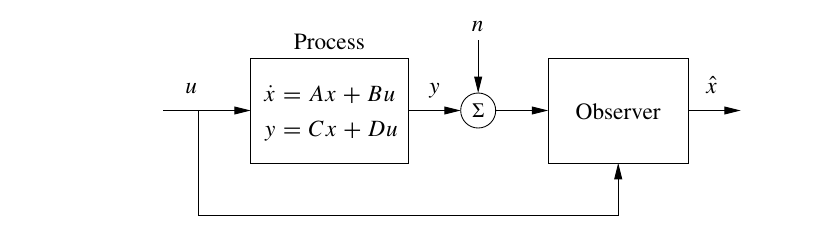
\includegraphics[scale=0.380]{img/output_feedback/observer_block_diagram.jpeg}
\end{center}
\caption{Block diagram for an observer. The observer uses the process measurement $y$
(possibly corrupted by noise $n$) and the input $u$ to estimate the current state of the process,
denoted $\hat{x}$.}
\label{observer_block_diagram}
\end{figure}


The problem of observability is one that has many important applications, even
outside feedback systems. If a system is observable, then there are no hidden dynamics inside it; we can understand everything that is going on through observation (over time) of the inputs and outputs. As we shall see, the problem of observability is of significant practical interest because it will determine if a set of sensors is
sufficient for controlling a system. Sensors combined with a mathematical model
can also be viewed as a virtual sensor that gives information about variables that
are not measured directly. The process of reconciling signals from many sensors
with mathematical models is also called sensor fusion.



\section{Testing for Observability}
\label{test_observability}

When discussing reachability in the last chapter, we neglected the output and focused on the state. Similarly, it is convenient here to initially neglect the input and
focus on the autonomous system



\begin{framed}
\theoremstyle{remark}
\begin{remark}{\textbf{Autonomous System}}

\end{remark}
\end{framed}

\begin{equation}
\frac{dx}{dt} = Ax ~~ y = Cx
\end{equation}

The objective is to understand when it is possible to determine the state from observations of the output. From

\begin{equation}
y = Cx
\end{equation}

we see that the output itself gives us the projection of the state $x$ on vectors that are rows of the matrix $C$. The 
observability problem can  immediately be solved if the matrix $C$ is invertible. If the matrix is not invertible we can take the derivatives and obtain

 
\begin{equation}
\frac{dy}{dt} = C\frac{dx}{dt} = CAx
\end{equation}

From the derivative of the output we thus get the projection of the state on vectors that are rows of the matrix $CA$. Proceeding in this way, we get

\begin{equation}
\begin{bmatrix}
 y \\
 y^{(1)} \\
 \vdots \\
 y^{(n-1)} 
\end{bmatrix} = 
\begin{bmatrix}
 C \\
 CA \\
 \vdots \\
 CA^{n-1} 
\end{bmatrix}x
\end{equation}

We thus find that the state can  be  determined if the observability matrix
 
\begin{equation}
W_o= 
\begin{bmatrix}
 C \\
 CA \\
 \vdots \\
 CA^{n-1} 
\end{bmatrix}
\end{equation}

has $n$ independent rows.  It turns out  that  we  need  not consider any derivatives higher
than $n-1$ (this is an application of the Cayley-Hamilton theorem)
 
\begin{framed}
\theoremstyle{remark}
\begin{remark}{\textbf{System with inputs}}

The calculation can easily be extended to systems with inputs. The state is then
given by a linear combination of inputs and outputs and their higher derivatives.
The observability criterion is unchanged. 
\end{remark}
\end{framed}


\begin{framed}
\theoremstyle{theorem}
\begin{theorem}{\textbf{Observability rank condition}}

A linear system of the form  
\begin{equation}
\frac{dx}{dt} = Ax + Bu, ~~ y = Cx + Du \nonumber
\end{equation}

is observable if and only if the observability matrix $W_o$ is full rank.
\end{theorem}
\end{framed}

\section{Observable Canonical Form}
\label{observability_canonical_form}

As in the case of reachability, certain canonical forms will be useful in studying ob-
servability. A linear single-input, single-output state space system is in observable
canonical form if its dynamics are given by


\begin{framed}
\theoremstyle{remark}
\begin{remark}{\textbf{Observable Canonical Form for Nonlinear Systems}}

The definition can be extended to systems with many inputs; the only difference is
that the vector multiplying u is replaced by a matrix.
\end{remark}
\end{framed}


The characteristic polynomial for a system in observable canonical form is

\begin{equation}
\lambda(s) = s^n +\alpha_1s^{n-1} + \ldots + \alpha_{n-1}s + \alpha_n
\end{equation}

In order to check the observability property of a systme more formally, we can compute the observability matrix for
a system in observable canonical form. This is given by

\begin{equation}
W_o= 
\begin{bmatrix}
 1 & 0 & 0 & \ldots &  0\\
 -\alpha_1 & 1 & 0 & \ldots &  0 \\
 -\alpha_{1}^{2} - \alpha_1 \alpha_2 & - \alpha_1 & 1 &  \ldots &  0 \\
 \vdots & \vdots & \vdots & \ddots & \vdots \\
* & * & * & \ldots & 1
\end{bmatrix} 
\end{equation}


where * represents  an entry  whose exact  value  is  not important.
What is important here is the rows of this matrix are linearly independent (since it is lower triangular), and hence Wo is full rank. Hence, it is invertible. 

As in the case of reachability (see section \ref{reachable_canonical_form}), it  turns  out  that  if a  system  is  observable then there
always exists a transformation $T$ that converts the system into observable canonical
form. This is useful for proofs since it lets us assume that a system is in observable
canonical form without any loss of generality. The observable canonical form may
be poorly conditioned numerically.
 

\section{State Estimation}
State feedback control design, as explained in t chapter \ref{state_feedback} requires that we have access to the complete state vector. 
However, measuring the complete state vector is not always feasible (for example a sensor may not be available at all) and it may also be expensive.
In this section we will introduce the idea of state estimation as a way to get access to the state variables. 


\begin{framed}
\theoremstyle{remark}
\begin{remark}{\textbf{Soft Sensors}}


The concept of using software instead of sensors to access the quantity we are 
interested in, is referred to as soft sensors in the automotive industry.
\end{remark}
\end{framed}

Recall that the idea of state feedback control was to modify the eigenvalues of the system under consideration by using the input

\begin{equation}
u = -Kx + K_r r  
\end{equation}

However, it can be seen that this requires the state vector $x$. The idea of state estimation is to design something called an observer that tries to provide an 
estimate say $\hat{x}$ of the state vector $x$. The observer is fed with the same input as the real plant. The goal of the observer is to provide somehow a replica of the true state vector.
Thus, we would like to have the error $\tilde{x}$ between the two quantities to be zero. Namely,


\begin{equation}
\tilde{x} = x - \hat{x} = 0 
\end{equation}
 
In this section, we want to construct a dynamical system of the form

\begin{equation}
\frac{d \hat{x}}{dt} = F\hat{x} + Gu + Hy  
\end{equation}

where $u$ and $y$ are the input and output of the original system and $\hat{x} \in R^n$ is an estimate of $x$ with the property

\begin{equation}
\hat{x}(t) \rightarrow x(t), ~~ \text{as} ~~ t \rightarrow \infty  
\end{equation}

Let's consider again the system

\begin{equation}
\frac{dx}{dt} = Ax + Bu ~~ y = Cx + Du
\label{sys}
\end{equation}

assume further that $D$ is zero. Assuming that the input $u$ is known, then an estimate of the state $x$ is given by

\begin{equation}
\frac{d\hat{x}}{dt} = A\hat{x} + Bu
\label{observer_one} 
\end{equation}  

We would like to know the properties of this estimate; how far is from the exact state? The estimation error is \cite{Astrom} 

\begin{equation}
\tilde{x} = x - \hat{x} 
\end{equation} 

substituting into equation \ref{observer_one} we find that


\begin{equation}
\frac{d\tilde{x}}{dt} = A\tilde{x}  
\end{equation}  

We already know that the behavior of this system depends on the eigenvalues of $A$. Concretely, if matrix $A$ has all its eigenvalues in the left half-plane, the error $\tilde{x}$ will go to zero,
and hence equation \ref{observer_one} is a dynamical system whose output converges to the state
of the system \ref{sys}.


The observer given by equation \ref{observer_one} uses only the process input $u$; the measured
signal does not appear in the equation. We must also require that the system be stable,
and essentially our estimator converges because the state of both the observer and
the estimator are going zero. This is not very useful in a control design context since
we want to have our estimate converge quickly to a nonzero state so that we can
make use of it in our controller. We will therefore attempt to modify the observer
so that the output is used and its convergence properties can be designed to be fast
relative to the system’s dynamics. This version will also work for unstable systems.

Let's now consider the following observer

\begin{equation}
\frac{d \hat{x}}{dt} = A\hat{x} + Bu + L(y- C \hat{x})
\label{observer_two}   
\end{equation}

The term $L(y- C \hat{x})$ provides feedback and hence the observer in \ref{observer_two} can be seen as a generalization of the observer in \ref{observer_one}. The supplied feedback is proportional to the difference between the observed output and the output predicted by the observer. Substituting the expression for the error $\tilde{x}$ we arraive at

 \begin{equation}
\frac{d\tilde{x}}{dt} = (A-LC)\tilde{x} 
\label{observer_two}   
\end{equation} 

If the matrix $L$ can be chosen in such a way that the matrix $A-LC$ has eigenvalues with negative real parts, the error $\tilde{x}$ will go to zero. The convergence rate is determined by an appropriate selection of the eigenvalues.
 

\begin{framed}
\theoremstyle{remark}
\begin{remark}{\textbf{Observer design and state feedback duality}}


Notice the similarity between the problems of finding a state feedback and
finding the observer. State feedback design by eigenvalue assignment is equivalent
to finding a matrix $K$ so that $A-BK$ has given eigenvalues. Designing an observer
with prescribed eigenvalues is equivalent to finding a matrix $L$ so that $A-LC$ has
given eigenvalues. Since the eigenvalues of a matrix and its transpose are the same
we can establish the following equivalences:

\begin{equation}
A \leftrightarrow A^T, ~~ B \leftrightarrow C^T, ~~ K \leftrightarrow L^T, ~~ W_r \leftrightarrow W_{o}^{T}
\end{equation}

The observer design problem is the dual of the state feedback design problem. 
\end{remark}
\end{framed}



\begin{framed}
\theoremstyle{theorem}
\begin{theorem}{\textbf{Observer design by eigenvalue assignment}}


Consider the system

\begin{equation}
\frac{dx}{dt} = Ax + Bu, ~~ y =Cx   \nonumber
\end{equation} 

with one input and one output. Let the characteristic polynomial related to matrix A be

\begin{equation}
\lambda(s) = s^n + \alpha_1 s^{n-1} + \ldots + \alpha_{n-1}s + \alpha_n \nonumber
\end{equation}

If the systme is observable, then the dynamical system

\begin{equation}
\frac{d \hat{x}}{dt} = A\hat{x} + Bu + L(y- C \hat{x})  \nonumber
\end{equation}


is an observer for the system with $L$ chosen as 

\begin{equation}
L = W_{o}^{-1}\tilde{W}_o
\begin{bmatrix}
 p_1 - \alpha_1 \\
 p_2 - \alpha_2 \\
 \vdots  \\
 p_n - \alpha_n
\end{bmatrix} \nonumber
\end{equation}

The matrices $W_{o}$ and $\tilde{W}_{o}$ are given by

The resulting observer error $\tilde{x}$ is governed by a differential equation that has the following characteristic polynomial

\begin{equation}
p(s) = s^n +  p-1 s^{n-1} + \ldots + p_n  \nonumber
\end{equation}
\end{theorem}
\end{framed}

The dynamical system (7.10) is called an observer for (the states of) the system (7.9) because it will generate an approximation of the states of the system from its inputs and outputs. This form of an observer is a much more useful form than the one given by pure differentiation in equation (7.3).


\section{Questions}

\textbf{Question 1}

What is the main reason for using an estimator in feedback control?

\begin{itemize}
\item A) There are process disturbances in the model 
\item B) We are measuring the wrong quantities 
\item C) It is too expensive or impractical to measure each state variable correct 
\end{itemize} 

\textbf{Answer}  

Option C is the correct answer.


\section{Answers to Questions}
\label{answer_questions}

{\textbf{Answer to questions in section \ref{introduction_self_driving_cars_questions}}}

\begin{enumerate}

\item Which of the following are components of longitudinal control? (Select all that apply)

\begin{itemize}
\item Braking and accelerating are components of longitudinal control. Thus, options 1 and 3 are correct
\end{itemize}

\item Which of the following is not an example of OEDR?

\begin{itemize}
\item Finding routes between locations is a long term planning problem and not OEDR. Hence, option 2 is correct.
\end{itemize}

\item Which of the following tasks would you expect a Level 2 system to perform? (Select all that apply)

\begin{itemize}
\item Options 1 and 3 are correct.
\end{itemize}

\item What is the distinction between Level 3 autonomy and Level 4 autonomy? 

\begin{itemize}
\item Option 4 is correct.  Level 3 systems cannot handle emergencies automatically and as a result require full user alertness.
\end{itemize}

\item What distinguishes Level 5 Autonomy from Level 4?

\begin{itemize}
\item Option 3 is correct. Level 5 systems can operate in any weather condition, on any road type or surface and in any scenario and remain safe.
\end{itemize}

\end{enumerate}

{\textbf{Answer to questions in section \ref{perception_questions}}}

\begin{enumerate}

\item Which of the following tasks are associated with perception? (Select all that apply) 
\begin{itemize}
\item Perception deals with position, motion estimation and object identification. Hence options 1 and 2 are correct.
\end{itemize}

\item Which of the following can be on road objects? (Select all that apply) 

\begin{itemize}
\item Potholes and vehicles are on road objects. So options 1 and 4 are correct.
\end{itemize}

\item Which of the following tasks pose challenges to perception? (Select all that apply) 

\begin{itemize}
\item All four choices pose challenges to perception
\end{itemize}

\item Which of the following sensors are used for ego localization? (Select all that apply) 


\begin{itemize}
\item Global Navigation Satellite System (GNSS) sensor provides position and velocity measurements, and can be used to estimate vehicle position and orientation for localization. An IMU provide acceleration and rotation rate measurements from accelerometers and gyroscopes, and can be used to estimate vehicle orientation and aid in localization in general. Thus, options 1 and four are correct.
\end{itemize}

\item Which of the following objects would be relevant for perception in adaptive cruise control?


\begin{itemize}
\item Adaptive cruise control detects vehicles ahead to control speed and to maintain safe driving distances. So
option 3 is correct. 
\end{itemize}

\end{enumerate}


\clearpage

\bibliographystyle{plain}
\input{references.bbl}
\end{document}
